\documentclass[12pt,a4paper]{article}
\usepackage[margin=2.5cm]{geometry}
\usepackage[utf8]{inputenc}
\usepackage[
    backend=biber,
    style=apa,
    citestyle=authoryear
]{biblatex}
\setlength{\bibitemsep}{0.5em}
\addbibresource{references.bib}
\usepackage{parskip}
\usepackage{xcolor}
\usepackage{graphicx} % Add this package for including images
\usepackage{hyperref} % Add this package for hyperlinks
\usepackage{caption} % Add this package for caption customization

\title{Multi-core Synergy: A Study of Performance Improvements Utilizing Multi-core Threading}
\author{J. Wolffrom}
\date{\today}

\begin{document}

\maketitle
\newpage

\begin{abstract}

\end{abstract}
\newpage

\tableofcontents
\newpage

\section{Disclosure}

Any and all resources related to- and used in this study can be found here:

\href{https://github.com/X1las/AsSynergy}{https://github.com/X1las/AsSynergy}

Due to the amount of variables that can affect the performance of a CPU, the results of this study should be taken in comparison to each other, and not as a definitive measure of performance. It is encouraged to run the code snippets on your own machine to get a better understanding of the performance improvements that can be achieved with multi-core threading.

In addition to this, this paper does fall within the scope of the Humanities and Technology department at the University of Roskilde, as it aims to understand how multi-core threading is being used in society today, and how it can be improved. More specifically, it falls within the dimension of Technological Systems and Artifacts (TSA) as we take a look at computer systems at large, and how people are using them- as well as how concepts within them are understood.

\section{Introduction}

Quoted by \cite{Rauber2023}, "Moore’s law is an empirical
observation which states that the number of transistors of a typical processor chip
doubles every 18 to 24 months. This observation has first been made by Gordon
Moore in 1965 and has been valid for more than 40 years. However, the transistor
increase due to Moore’s law has slowed down during the last years" 

\citeauthor{Rauber2023} posits that the number of transistors on a microchip used to double rougly every two years, leading to an exponential increase in computing power. However they, in accordance with \cite{Mattson2014}, agree that this trend has been dwindling since some time around 2005, as a limit was reached on how many transistors could be placed on a single computer chip without overheating and damaging the circuitry. Even by utilizing the most advanced tricks and optimizations available, the performance improvements we are seeing annually as of 2023 are somewhere around 3.5\% faster CPU clock speeds \parencite[p. 11]{Rauber2023} which is a far cry from the 50\% annual increases we were seeing in the early 2000's \parencite[p. 11]{Rauber2023}. 

As a result of the processing speed ceiling, the focus has shifted from increasing the clock speeds of CPUs to adding more computational units to them. This has led to a rise in multi-core processors, which contain multiple processing units on a single CPU chipset, often referred to as "cores". These cores can execute multiple orders simultaneiously, which can lead to significant performance improvements in software applications. However, a discrepancy can be found in the communities that rely on these improvements. An article from IGN \parencite{Thomas2025} on picking optimal hardware for computer games describes it best:

\begin{quote}
    \textit{\textcolor{darkgray}{"While there are some PC games that love CPUs with a dozen or more cores, they’re few and far between. 
    Instead, finding an 8-core, 16-thread processor with a high clock speed and a lot of L3 Cache is going to get you further than just adding more CPU cores to the equation". }}
\end{quote}

A trend of diminishing returns can be seen, or rather felt on a consumer basis. Even people who purchase CPUs know to steer away from something that advertises a high amount of cores, as it's simply not worth it. Whereas the relationship between core-count and performance we should be seeing, in theory, should be an equivalence. It is evident that traditional single-core processors are opting out of the market in place of processors with more and more cores \parencite{Smith2023}, but the performance improvements are not being felt by the end-user.

\subsection{The Problem Area}

If multi-core threading is the future, then it is essential to understand why it is not delivering the expected performance improvements it has the potential to deliver. \cite[p. 12]{Rauber2023} mentions that simulations have shown that superscalar processors with up to four functional units yield substantial benefits over the use of a single functional unit. So in theory, it would seem there is a great potential to gain from utilizing multiple cores. Some of it has been utilized according to \textcite{Thomas2025}, as we are talking about 8-cores as opposed to one, but it has taken us 20 years to get to this point.

As such, this study aims to address this question of why multi-core optimization is so difficult to accomplish, if and/or how it can be improved, and what the potential benefits of doing so are. 

\subsubsection{Research Question}

This being said, there are limits to what can be achieved in such a short study, therefore we will be focusing on threads and schedulers. The way to implement them, as well as how different programming languages handle them. This will be done by looking at the different threading libraries available in C, C\#, Java and Python, as well as the different schedulers that are used to manage them.

The research question that we will be addressing is then as follows:

\begin{quote}
    \textit{What does multi-core threading performance look like, and how do different schedulers affect it?}
\end{quote}

This question can then be further broken down into the following sub-questions:

\begin{itemize}
    \item What is a thread and how do you use it?
    \item What is a scheduler and does where does it differentiate between systems and programming languages?
    \item What performance increases and deficits does multi-core threading incur?
    \item What are the challenges of multi-core threading, and how can they be overcome?
\end{itemize}

These questions serve to guide the study as a framework, outlining the key areas we need to understand in order to answer the main research question at large. But with that being said, we will be limiting the scope of this study in order to have a deeper understanding of the subject matter within their short confines.

\subsubsection{Limitations}

This study is limited in its research and data-collection to only a handful of programming languages: C, C\#, Java and Python. This is due to the fact that these languages are the most commonly used in the field of computer science, and therefore provide a lot of insight into the subject matter that is relevant to the readers. Whilst also common, they all handle multi-core threading in wildly different ways, which allows us to trace the remnants of different threading architectures and how they affect the performance of multi-core threading.

This being said, we will not delve into the specifics of each language, but rather focus on the threading libraries and how they are used in practice. This is to ensure that we can provide a comprehensive overview of the subject matter without getting bogged down in the details of each language.

Additionally, this study limits its operating system scope to just Linux, as this was the easiest method of collecting data. This is due to linux having a lot of built-in tools and easy-to-install features that allowed for easy programming in all 4 different languages. This is not to say that the results are not applicable in other operating systems, in fact we encourage the reader to run the code snippets on a windows environment to see if the results are similar- However, we will not be able to provide any data on this, as it was not part of the study.

In addition to this, we will also only be talking about x64 architecture, as this is the most common architecture used in modern computers, and the architecture used in both the Intel and AMD processors tat most Windows and Linux machines run on. For the purpose of this study, we will only be looking at Intel processors, as they are the components readily available to us for testing. This is not to say that the results are not applicable to AMD processors, but we will not be able to provide any data on this, as it was not part of the study.

\section{Asynchronous Systems}

To understand multi-core systems effectively, we must first differentiate between synchronous and asynchronous execution paradigms. These concepts form the foundation for how tasks are distributed and managed across multiple processing units.

In traditional single-core processing, operations follow a synchronous model where instructions execute sequentially in a predetermined order \parencite[p. 118]{Johnson2015}. This means that each instruction must complete before the next one begins, creating a linear flow of execution. This model is straightforward and easy to understand, but even on a single-core processor there is still a need the need for running multiple processes at the same time. In addition to this, it's also inefficient to wait for one process to finish entirely before starting the next one, leading to the processor "idling" whilst waiting for I/O operations or resources to become available.

\begin{quote}
    \textit{\textcolor{darkgray}{"It is much easier to reason sequentially, doing only one thing at a time, than to understand situations where many things occur simultaneously." ... "Thus, while we are “parallel processors”, and we live in a world where multiple things happen at the same time, we usually reason by reduction to a sequential world."}} - \cite{Rajsbaum2020}
\end{quote}

This creates a need for switching the processors attention, or "context switching" between different tasks, which is a key feature of modern operating systems. This allows the processor to switch between different tasks quickly, giving the illusion of everything running at the same time, also known as "concurrency"\parencite{Rajsbaum2020}. This is a common approach in single-core systems, where the operating system manages the execution of multiple processes by rapidly switching between them. This is often done using a time-slicing technique, where each process is given a small time slice to execute before the processor switches to the next one.

\subsection{Subroutines and Coroutines}

This is often seen by the programmer in the form of subroutines, which in layman's terms are just functions \parencite{Pyeatt2020}, a piece of code that can be called from anywhere in the program. This is a common approach in programming that most, if not all programmers are familiar with, where functions are used to encapsulate a specific piece of functionality and can be called from anywhere in the program, and often multiple times. This allows for code reuse and modularity, making it easier to write and maintain complex programs, but by expanding them to coroutines we can achieve a lot more, namely Concurrency and Asynchronousity. 

Coroutines carry an additional layer of complexity, as they allow for the suspension and resumption of execution at specific points \parencite{DeMouna2009}. This means that a coroutine can "yield" control back to the calling code, before finishing its execution, allowing for more complex interactions between different parts of the program. This is often used in asynchronous programming, where coroutines can be used to handle I/O operations without blocking the main process. 

Depending on how Coroutines are used, they can be either synchronous or asynchronous. In a synchronous coroutine, the coroutine will yield control back to the calling code, but will not return until it has finished executing. This means that the calling code will wait for the coroutine to finish before continuing. In an asynchronous coroutine, the coroutine will yield control back to the calling code, and will return immediately, allowing the calling code to continue executing.

This suspension and resumption capability is often expressed through 'yield' and 'resume' operations, enabling coroutines to implement cooperative multitasking patterns where execution flow can be transferred between different tasks without requiring them to complete first.

For an example, look at the following python snippet:
\begin{verbatim}

import asyncio

async def main():
    print('Hello ...')
    await asyncio.sleep(1)
    print('... World!')

asyncio.run(main())
\end{verbatim}

Which defines an asynchronous main function, or a coroutine that will print "Hello World" interspaced by one second. This shows the prominent 'yield' operation. If we gave the function a target to yield to, we would in turn make the code "synchronous" in nature.

When expanding to multiple processing units on the same chipset (a multi-core processor), we can maintain this synchronous approach for consistency or adopt an asynchronous model that allows processing units to operate with greater independence. 

In practice, synchronous and asynchronous models are rarely implemented in their purest forms. Even highly parallel systems require synchronization mechanisms to coordinate access to shared resources. For instance, memory access operations must be coordinated when multiple cores need to read from or write to the same memory locations simultaneously. Even when we believe to have written a purely synchronous program, the underlying hardware and operating system may still introduce asynchronous behavior through context switching and resource management because of the need for concurrency.

\section{Threading}

The reason why subroutines and coroutines are important to understand is because they relate quite heavily to how threads operate. In fact, a thread is in essense a coroutine that is managed by the operating system, allowing for multiple threads to be executed concurrently. This means that threads can be used to execute multiple tasks at the same time, without blocking the main process.

Threading is a way of executing multiple different tasks at the same time in a computer operating system. Every program on a computer intrinsically define at least one thread of operations they want the operating system to execute. This is often referred to as the main thread, and is the thread that is executed first when a program is started, which can then spawn sub-threads to execute other tasks. The OS then handles what order threads are executed in using what is known as a "Scheduler", this scheduler is then also responsible for 'Suspending' threads to make it seem like all programs are executed concurrently. 

This process of suspending threads is what allows for the illusion of concurrency, allowing the operating system to seemingly execute multiple threads at the same time by switching back and forth rapidly between tasks. This is known as "context switching", and is a key feature of modern operating systems, making even a single core processing system capable of multi-tasking.

This is not to be confused with multi-core processing, which is the ability to execute multiple threads at the same time with different cores. This is where the real performance improvements come from, as we can execute multiple tasks at the same time without having to switch as often.

\subsection{Threading in different languages}

\subsubsection{Posix}

Posix is a standard for multi-core threading in C, and comes pre-installed with unix systems such as Linux in the GCC compiler used for this study. It is a library that provides a set of functions for creating and managing threads, as well as synchronizing access to shared resources. This means that Posix is able to utilize multiple cores in a program, but it is not as easy to implement as it is in other languages.

\subsubsection{Threading in C}

C, unlike the previous mentions, is a low-level programming language. It is a compiled language that is designed to be fast and efficient, making it a popular choice for system programming and embedded systems. C is often used in applications where performance is critical, such as operating systems, device drivers, and high-performance computing, as well as game engines. It is therefore a prime candidate for multi-core processing optimization, as wherever C is used in practice it is often done so with performance in mind.

C provides a library for multi-core threading called Posix, labeling their way of threading as 'pthreads' or 'POSIX threads'. This library is a standard for multi-core threading in C, and comes pre-installed with unix systems such as Linux in the GCC compiler used for this study.

\subsubsection{Threading in C-Sharp}

C\# is a compiled language that is part of the C language family like Python, however where it differs is its striking resemblance to Java. It is a high-level language that is designed to be easy to use and understand, gathering a lot of attention due to its usage in the Unity game engine as well as developers transitioning from other languages. It is therefore a prime candidate for multi-core processing optimization as Java developers come potentially pre-equipped with a solid foundation of threading, as well as new game developers looking for performance improvements.

The way C\# handles multi-core threading is not the same as Java, as it provides a library to assign tasks to threads, which in turn are managed by the operating system's scheduler. This means that C\# is able to utilize multiple cores in a program, but it is not as easy to implement as it is in Java. However, C\# does have some advantages over Java when it comes to performance, as it is a compiled language and therefore faster than Java. In addition, C\# has a more efficient memory management system than Java, which can lead to performance improvements in large programs.

\subsubsection{Threading in Python}

As it stands, Python is one of the most popular programming languages in the field of computer science. It is widely used in a variety of applications due to its simplicity and ease of use. However, it is an interpreted language, which means that it is not as fast as compiled languages like C or C++. In fact it is written in C, which is a compiled language. This means that in places it keeps the speed of C by pre-compiling certain commands, but in other places it is slower than C, with up to 10 times the execution in difference.

This is important due to the way Python handles multi-core threading. By default, Python comes pre-installed with threading and asynchronous libraries, which allow for the use of multiple threads in a program, however the presence of the Global Interpreter Lock (GIL) means that only one core will be in use at any time. This means that the performance improvements of multi-core threading are not easily accessed, but by using libraries such as 'multiprocessing' or 'numpy', we can bypass the GIL using some of the same utilities in C. This allows us to use multiple cores in a program, but it is not as easy to implement as it is in other languages.

\subsubsection{Threading in Java}

Java comes with a built-in threading library, which allows for the use of multiple threads in a program, managed by the Java Virtual Machine (JVM). Usually this is accomplished by inheritance, designating a class as a thread, allowing it to use common threading methods such as sleep (suspension) and join (synchronization). This means that Java is able to utilize multiple cores in a program by use of their own scheduler, and the performance improvements are easily accessible. However, this is not without its drawbacks, as the JVM is an interpreted language, which means that it is not as fast as compiled languages like C or C++. In addition, the JVM is not as efficient as other languages when it comes to memory management, which can lead to performance issues in large programs. 

\section{Parallelism}

This ability to execute multiple tasks simultaneously with multiple cores is known as "parallelism". In this section we will be looking at notable terms and concepts that are important to understand when working with multi-core systems.

\subsection{Degree of Parallelism}

In the field of parallel systems architecture we often talk about the degree of parallelism a system is capable of. This is a measure of how many tasks can be executed at the same time, and is often used to describe the performance improvements that a parallel system provides.

This, in turn, coincides with the concept of "Potential Parallelism", which is the theoretical maximum degree of parallelism that a system can achieve. This is often used to describe the performance improvements that a parallel system can provide, and is often used as a benchmark for comparing different systems.

\subsection{Thread Level Parallelism (TLP)}

\subsection{Schedulers}

Schedulers are the part of the operating system that is responsible for managing the execution of threads. They are responsible for deciding which thread to execute at any given time, and for managing the resources that are used by each thread. This includes managing the CPU, memory, and other resources that are used by the threads. The scheduler is responsible for ensuring that each thread gets a fair share of the resources, and that no single thread is allowed to monopolize the resources.

Schedulers are often implemented as part of the operating system kernel, and are responsible for managing the execution of all threads in the system. This includes managing the scheduling of threads, as well as managing the resources that are used by each thread. The scheduler is responsible for ensuring that each thread gets a fair share of the resources, and that no single thread is allowed to monopolize the resources.

\subsubsection{OS Schedulers}


\subsubsection{.NET}

The .NET framework is a software development platform developed by Microsoft. It provides a large library of pre-built functions and classes that can be used to create applications for Windows and other platforms. The .NET framework includes a built-in threading library, which allows for the use of multiple threads in a program, managed by the .NET runtime. This means that the .NET framework is able to utilize multiple cores in a program, but it is not as easy to implement as it is in other languages.

\subsubsection{JVM}

The Java Virtual Machine (JVM) is a software-based execution environment that allows Java programs to run on any platform that has a JVM installed. The JVM is responsible for managing the execution of Java programs, including the creation and management of threads. This means that the JVM is able to utilize multiple cores in a program, but it is not as easy to implement as it is in other languages.

\subsection{Parallel Execution Time (PET)}

In this context of degrees of parallelism, we often use measures such as "Parallel Execution Time" (PET) to quantitatively describe the time it takes for a parallel system to execute a given task. 

This execution time is measured across all functional units, or cores of a system, and can be used to give a tangible measure of the running time of a parallel program. This means that waiting times for memory fetching, writing and plain idle times are included in the measure.

In terms of coding with multi-core threading, this means that "scheduling" time is included in the measure as well, as this is the time it takes for the operating system to assign tasks to different cores. This is important to note, as it means that the performance improvements of a parallel system are not just determined by the number of cores, but also by the efficiency of the scheduling algorithm used by the operating system.

\subsection{Load Balancing}

The term "Load Balancing" refers to the standard process of distributing tasks across multiple cores in a parallel system, such that tasks are executed equally across all cores. This is important to ensure that all cores are utilized effectively, and that no single core is overloaded with tasks while others are idle.

To this, it is important to note that not all cores are created equal, and that in terms of cpu-architecture we see a lot of variation with "Performance" and "Optional" cores. Performance cores are designed to handle heavy workloads, while optional cores are designed to handle lighter workloads. This means that load balancing is not just about distributing tasks evenly across all cores, but also about ensuring that the right tasks are assigned to the right cores. 

Even within the same core type we can see a lot of variation in terms of performance, as some cores are designed to handle specific tasks better than others. This is known as "heterogeneous computing", and is an important consideration when designing parallel systems, but as mentioned earlier, in this paper we will only deal with intel x64 architecture.

\subsection{Idle Time}

The time a processor cannot do anything useful but wait for more work.

\section{Memory}

\subsection{Shared Memory}

Memory organization where the machine shares memory for all threads.

Synchronization plays a heavy role, for example by keeping threads from reading files before another has written to them.

Often connected to the term "Thread".

\subsection{Local Caching}

\subsection{Memory Access Time (MAT)}

Add content if applicable.

\section{Further Reading}

efficiency cores vs performance cores

\section{Data Collection}

\subsection{Experiment Setup}

Before we get into the benchmarks of the different programming languages, it is important to disclose that the data was collected on a computer running Ubuntu 24.04.2 LTS with an intel Core i5-4460 CPU @ 3.2GHz, with 4 cores and 4 threads. The time measured was done so with various clocking methods depending on the programming language over the course of 5 runs, with the average time being taken as the final result. The code snippets used for the benchmarks can be found in the appendix.

To begin with, we clocked the time it took to execute a simple count from 1 to 1 billion in the various languages to get a frame of references. This proved especially difficult for Java, as the JIL converts commonly used methods to bytecode to optimize the execution time. This meant that to get a proper benchmark we had to disable the JIT compiler by using the '-Xint' flag, which in turn made the execution time of Java significantly slower than the other languages, with the exception of Python.

\newpage
\subsection{Results}

As expected, the results of running the code snippets in multiple cores were significant performance increases, as comared to the single core. This makes sense, as evidently four cores are faster than one, however some of these results were quite surprising.

\begin{figure}[!htb]
    \centering
    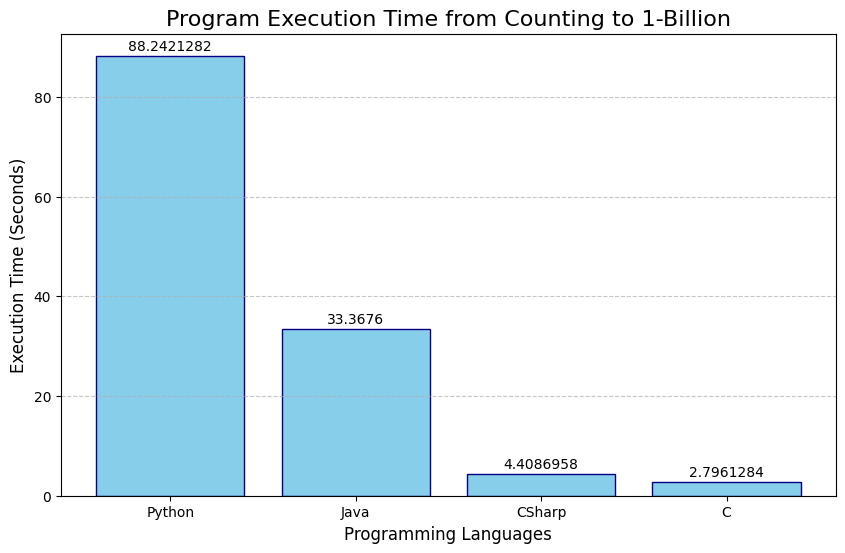
\includegraphics[width=0.8\textwidth]{../sync_records/sync_exec_times.png}
    \captionsetup{font=tiny, justification=centering}
    \caption{Execution time comparison of different programming languages running synchronously when counting from 1 to 1-billion.}
    \label{fig:sync-exec-times}
\end{figure}


The synchronous execution results above benchmark the time it took to compute the same task in each of the language. We saw expected results within most of the languages, with python having an average run time of 88 seconds, Java at 33, C\# 4 and C at a little less than 3 seconds. There was not much to note in these results, other than Java operating surprisingly slow when not using the JIT compiler.


\begin{figure}[!htb]
    \centering
    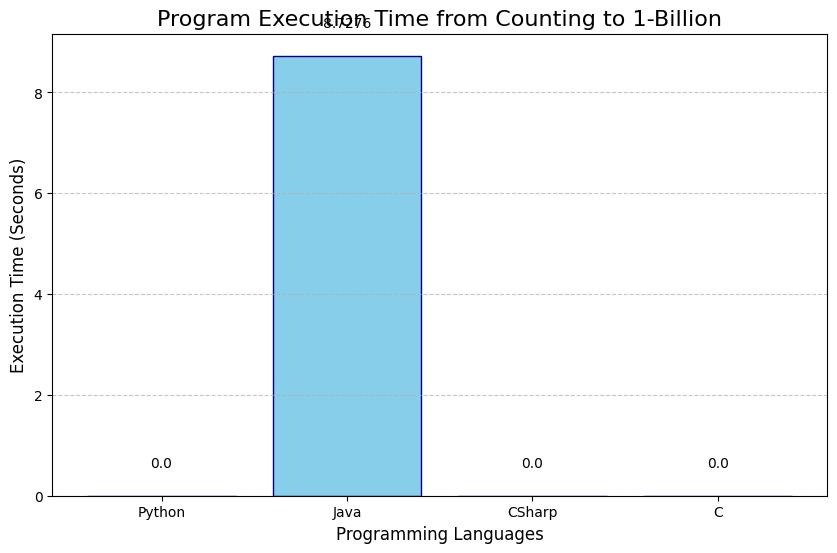
\includegraphics[width=0.8\textwidth]{../async_records/async_exec_times.png}
    \captionsetup{font=tiny, justification=centering}
    \caption{Execution time comparison of different programming languages running asynchronously with multi-threading when counting from 1 to 1-billion.}
    \label{fig:async-exec-times}
\end{figure}

The asynchronous execution results reveal a great deal about the efficiency of the different programming when using multiple cores. Python was able to achieve a time of 43 seconds on average which amounts to a little more than twice the performance increase. Java was able to achieve an astounding 8.7 seconds, a little less than 4 times the performance increase.

\newpage
\section{Discussion}

Include thoughts about other programming languages.

\newpage
\section{Conclusion}

Add content if applicable.

\newpage
\section{References}
\printbibliography
% Ensure Biber is run to resolve undefined references

\clearpage
\appendix

\section{Asynchronous Run-time Snippets}

\subsection{C Code Execution Times} 

\begin{figure}[htbp]
    \centering
    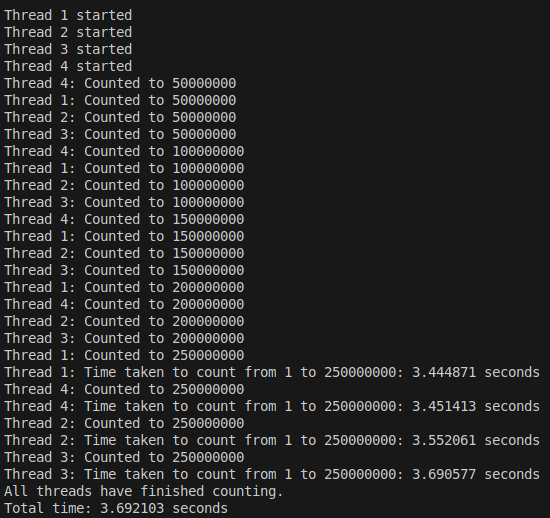
\includegraphics[width=0.8\textwidth]{../async_records/results_c/result_1.png}
    \caption{First run of asynchronous C code execution.}
    \label{fig:C-async-runtime-1}
\end{figure}

\begin{figure}[htbp]
    \centering
    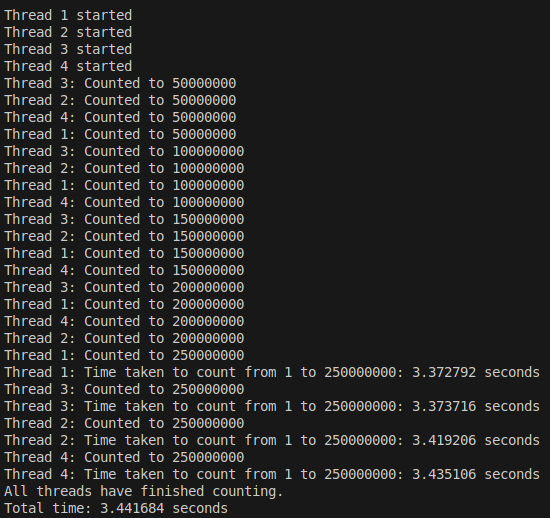
\includegraphics[width=0.8\textwidth]{../async_records/results_c/result_2.png}
    \caption{Second run of asynchronous C code execution.}
    \label{fig:C-async-runtime-2}
\end{figure}

\begin{figure}[htbp]
    \centering
    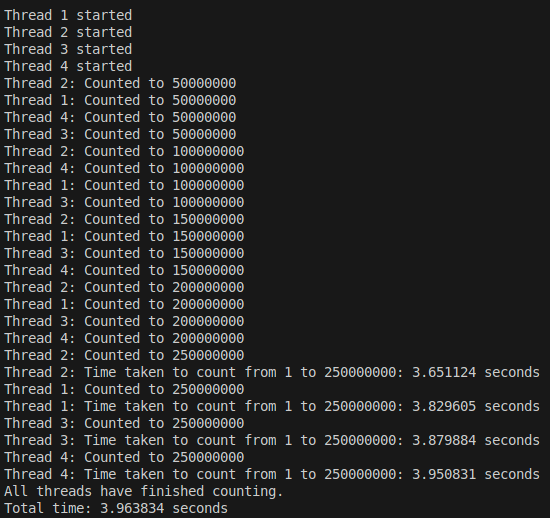
\includegraphics[width=0.8\textwidth]{../async_records/results_c/result_3.png}
    \caption{Third run of asynchronous C code execution.}
    \label{fig:C-async-runtime-3}
\end{figure}

\begin{figure}[htbp]
    \centering
    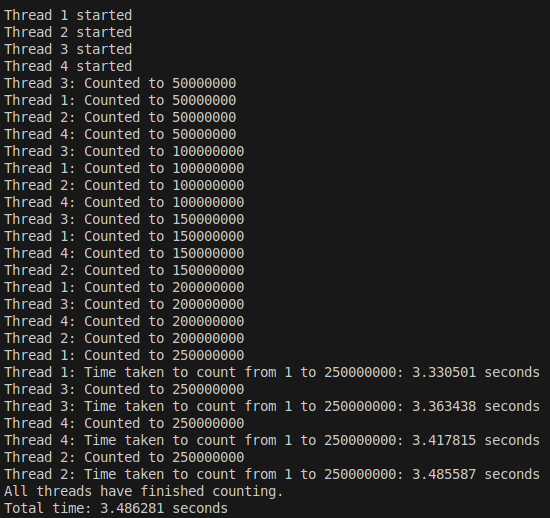
\includegraphics[width=0.8\textwidth]{../async_records/results_c/result_4.png}
    \caption{Fourth run of asynchronous C code execution.}
    \label{fig:C-async-runtime-4}
\end{figure}

\begin{figure}[htbp]
    \centering
    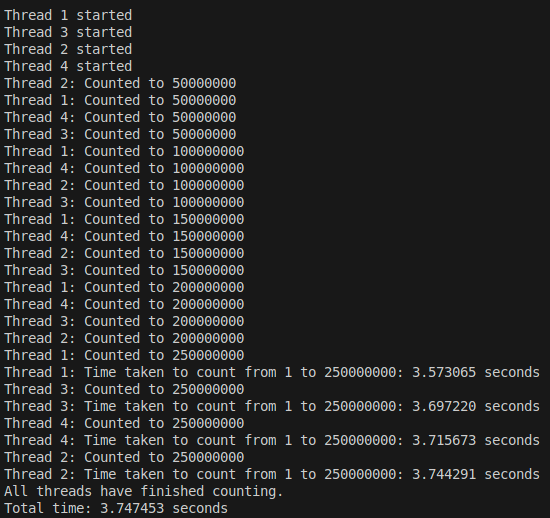
\includegraphics[width=0.8\textwidth]{../async_records/results_c/result_5.png}
    \caption{Fifth run of asynchronous C code execution.}
    \label{fig:C-async-runtime-5}
\end{figure}

\clearpage
\subsection{C-Sharp Code Execution Times} 

\begin{figure}[htbp]
    \centering
    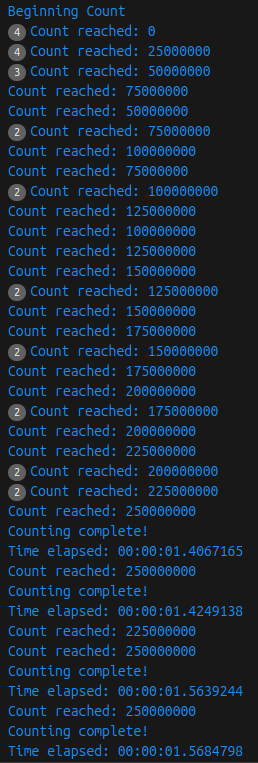
\includegraphics[width=0.8\textwidth]{../async_records/results_cs/result_1.png}
    \caption{First run of asynchronous C-Sharp code execution.}
    \label{fig:C-Sharp-async-runtime-1}
\end{figure}

\begin{figure}[htbp]
    \centering
    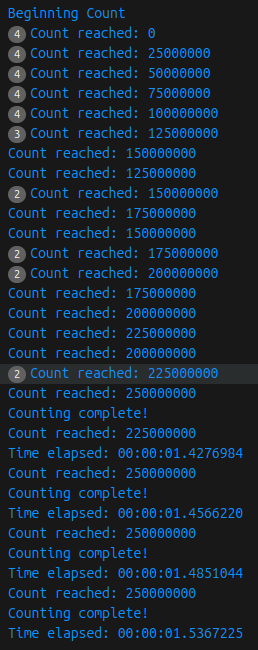
\includegraphics[width=0.8\textwidth]{../async_records/results_cs/result_2.png}
    \caption{Second run of asynchronous C-Sharp code execution.}
    \label{fig:C-Sharp-async-runtime-2}
\end{figure}

\begin{figure}[htbp]
    \centering
    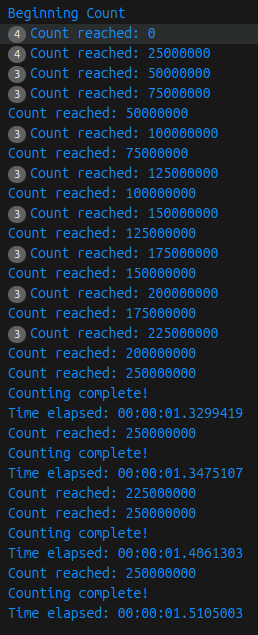
\includegraphics[width=0.8\textwidth]{../async_records/results_cs/result_3.png}
    \caption{Third run of asynchronous C-Sharp code execution.}
    \label{fig:C-Sharp-async-runtime-3}
\end{figure}

\begin{figure}[htbp]
    \centering
    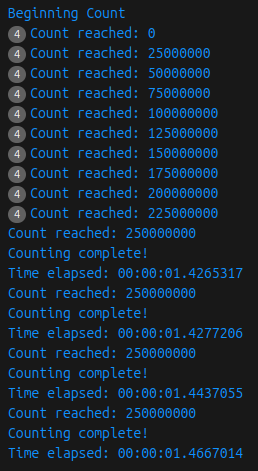
\includegraphics[width=0.8\textwidth]{../async_records/results_cs/result_4.png}
    \caption{Fourth run of asynchronous C-Sharp code execution.}
    \label{fig:C-Sharp-async-runtime-4}
\end{figure}

\begin{figure}[htbp]
    \centering
    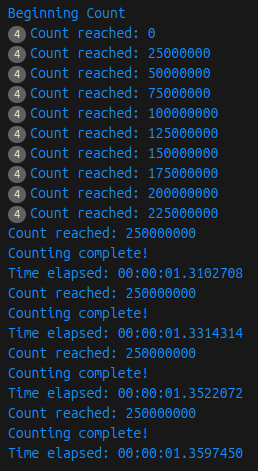
\includegraphics[width=0.8\textwidth]{../async_records/results_cs/result_5.png}
    \caption{Fifth run of asynchronous C-Sharp code execution.}
    \label{fig:C-Sharp-async-runtime-5}
\end{figure}

\clearpage
\subsection{Java Execution Times} 

\begin{figure}[htbp]
    \centering
    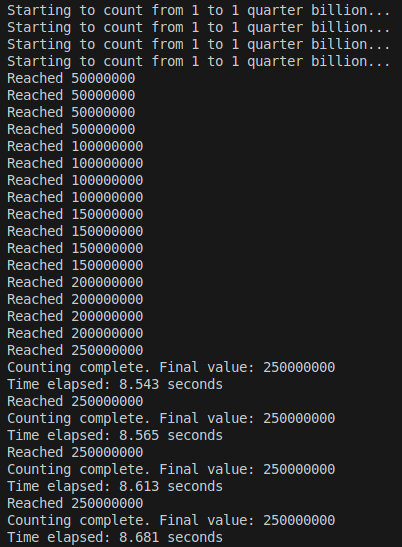
\includegraphics[width=0.8\textwidth]{../async_records/results_java/result_1.png}
    \caption{First run of asynchronous Java code execution.}
    \label{fig:Java-async-runtime-1}
\end{figure}

\begin{figure}[htbp]
    \centering
    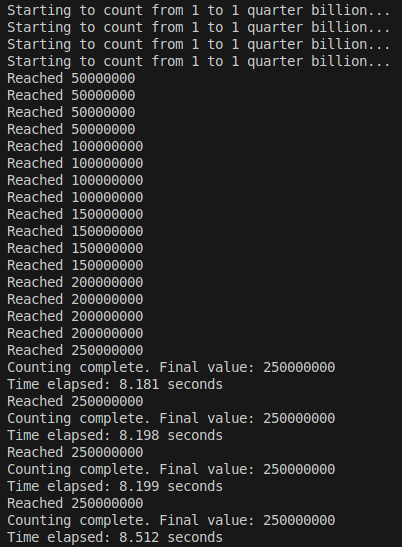
\includegraphics[width=0.8\textwidth]{../async_records/results_java/result_2.png}
    \caption{Second run of asynchronous Java code execution.}
    \label{fig:Java-async-runtime-2}
\end{figure}

\begin{figure}[htbp]
    \centering
    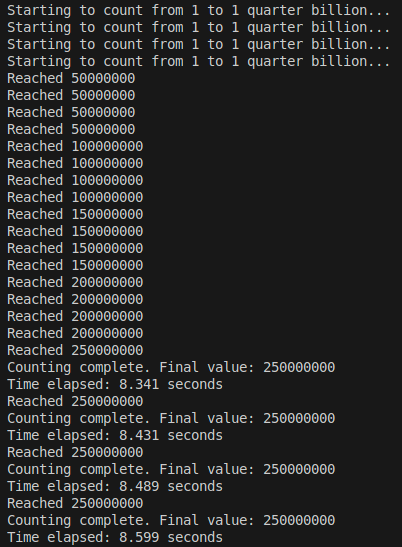
\includegraphics[width=0.8\textwidth]{../async_records/results_java/result_3.png}
    \caption{Third run of asynchronous Java code execution.}
    \label{fig:Java-async-runtime-3}
\end{figure}

\begin{figure}[htbp]
    \centering
    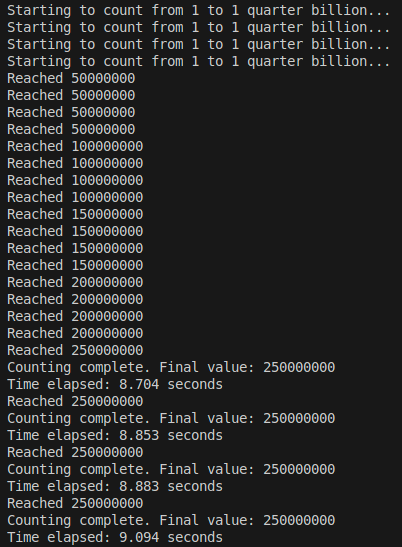
\includegraphics[width=0.8\textwidth]{../async_records/results_java/result_4.png}
    \caption{Fourth run of asynchronous Java code execution.}
    \label{fig:Java-async-runtime-4}
\end{figure}

\begin{figure}[htbp]
    \centering
    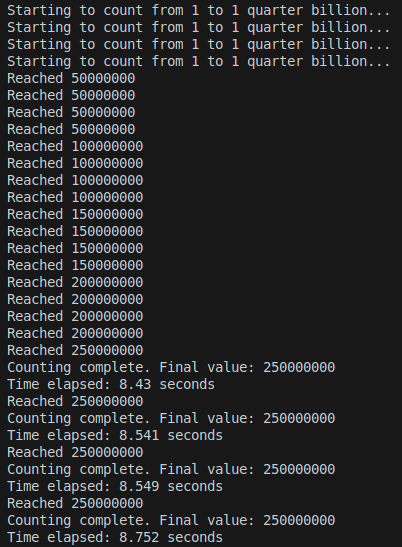
\includegraphics[width=0.8\textwidth]{../async_records/results_java/result_5.png}
    \caption{Fifth run of asynchronous Java code execution.}
    \label{fig:Java-async-runtime-5}
\end{figure}

\clearpage
\subsection{Python Execution Times} 

\begin{figure}[htbp]
    \centering
    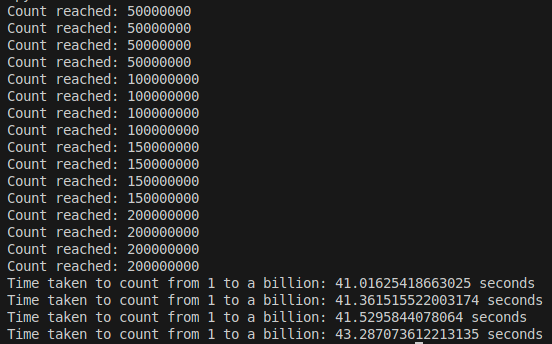
\includegraphics[width=0.8\textwidth]{../async_records/results_python/result_1.png}
    \caption{First run of asynchronous Python code execution.}
    \label{fig:Python-async-runtime-1}
\end{figure}

\begin{figure}[htbp]
    \centering
    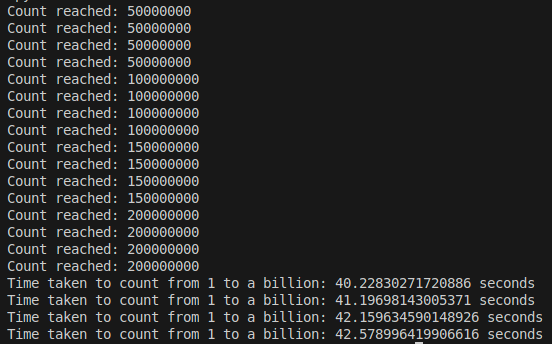
\includegraphics[width=0.8\textwidth]{../async_records/results_python/result_2.png}
    \caption{Second run of asynchronous Python code execution.}
    \label{fig:Python-async-runtime-2}
\end{figure}

\begin{figure}[htbp]
    \centering
    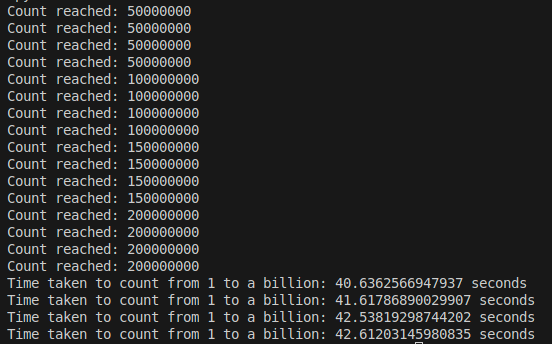
\includegraphics[width=0.8\textwidth]{../async_records/results_python/result_3.png}
    \caption{Third run of asynchronous Python code execution.}
    \label{fig:Python-async-runtime-3}
\end{figure}

\begin{figure}[htbp]
    \centering
    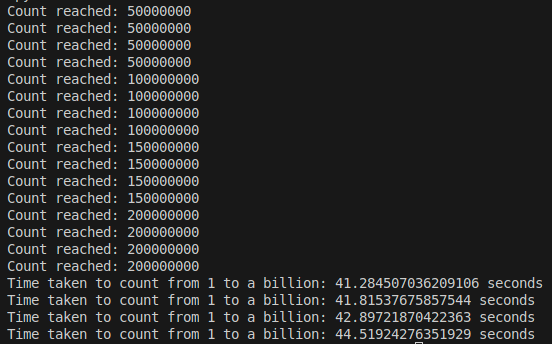
\includegraphics[width=0.8\textwidth]{../async_records/results_python/result_4.png}
    \caption{Fourth run of asynchronous Python code execution.}
    \label{fig:Python-async-runtime-4}
\end{figure}

\begin{figure}[htbp]
    \centering
    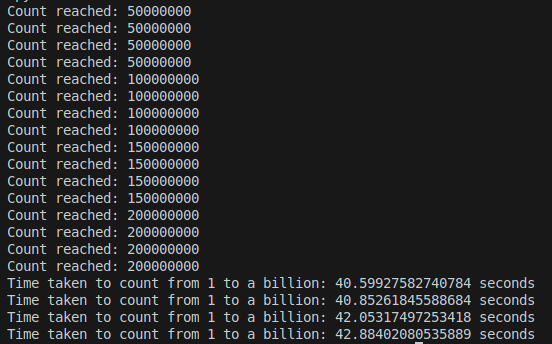
\includegraphics[width=0.8\textwidth]{../async_records/results_python/result_5.png}
    \caption{Fifth run of asynchronous Python code execution.}
    \label{fig:Python-async-runtime-5}
\end{figure}

\clearpage
\section{Synchronous Run-time Snippets}

\subsection{C Code Execution Times} 

\begin{figure}[htbp]
    \centering
    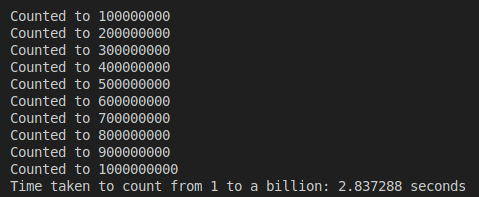
\includegraphics[width=0.8\textwidth]{../sync_records/results_c/result_1.png}
    \caption{First run of synchronous C code execution.}
    \label{fig:C-runtime-1}
\end{figure}

\begin{figure}[htbp]
    \centering
    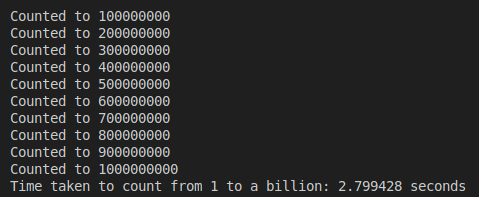
\includegraphics[width=0.8\textwidth]{../sync_records/results_c/result_2.png}
    \caption{Second run of synchronous C code execution.}
    \label{fig:C-runtime-2}
\end{figure}

\begin{figure}[htbp]
    \centering
    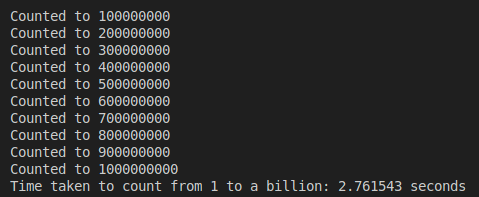
\includegraphics[width=0.8\textwidth]{../sync_records/results_c/result_3.png}
    \caption{Third run of synchronous C code execution.}
    \label{fig:C-runtime-3}
\end{figure}

\begin{figure}[htbp]
    \centering
    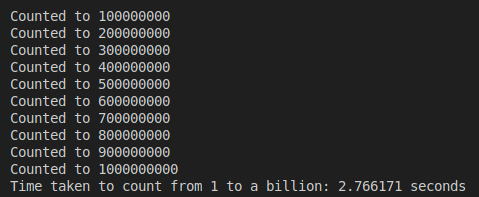
\includegraphics[width=0.8\textwidth]{../sync_records/results_c/result_4.png}
    \caption{Fourth run of synchronous C code execution.}
    \label{fig:C-runtime-4}
\end{figure}

\begin{figure}[htbp]
    \centering
    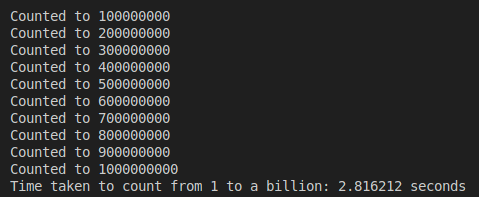
\includegraphics[width=0.8\textwidth]{../sync_records/results_c/result_5.png}
    \caption{Fifth run of synchronous C code execution.}
    \label{fig:C-runtime-5}
\end{figure}

\clearpage
\subsection{C-Sharp Code Execution Times} 

\begin{figure}[htbp]
    \centering
    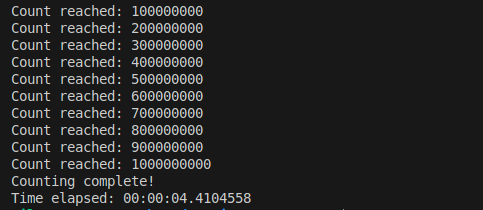
\includegraphics[width=0.8\textwidth]{../sync_records/results_cs/result_1.png}
    \caption{First run of synchronous C-Sharp code execution.}
    \label{fig:C-Sharp-runtime-1}
\end{figure}

\begin{figure}[htbp]
    \centering
    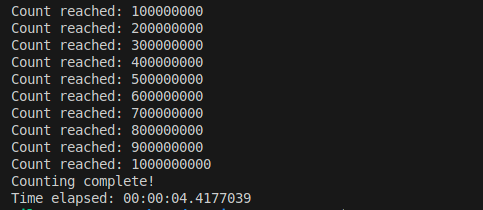
\includegraphics[width=0.8\textwidth]{../sync_records/results_cs/result_2.png}
    \caption{Second run of synchronous C-Sharp code execution.}
    \label{fig:C-Sharp-runtime-2}
\end{figure}

\begin{figure}[htbp]
    \centering
    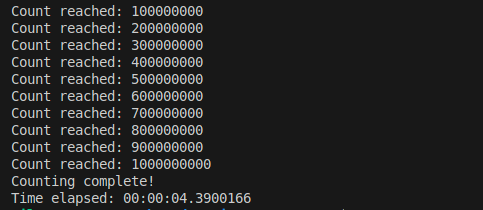
\includegraphics[width=0.8\textwidth]{../sync_records/results_cs/result_3.png}
    \caption{Third run of synchronous C-Sharp code execution.}
    \label{fig:C-Sharp-runtime-3}
\end{figure}

\begin{figure}[htbp]
    \centering
    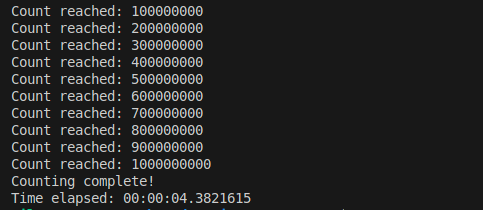
\includegraphics[width=0.8\textwidth]{../sync_records/results_cs/result_4.png}
    \caption{Fourth run of synchronous C-Sharp code execution.}
    \label{fig:C-Sharp-runtime-4}
\end{figure}

\begin{figure}[htbp]
    \centering
    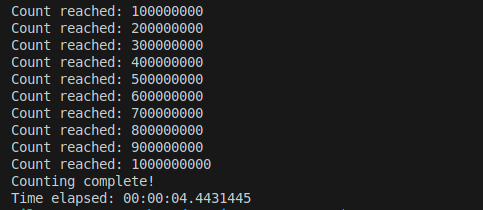
\includegraphics[width=0.8\textwidth]{../sync_records/results_cs/result_5.png}
    \caption{Fifth run of synchronous C-Sharp code execution.}
    \label{fig:C-Sharp-runtime-5}
\end{figure}

\clearpage
\subsection{Java Execution Times} 

\begin{figure}[htbp]
    \centering
    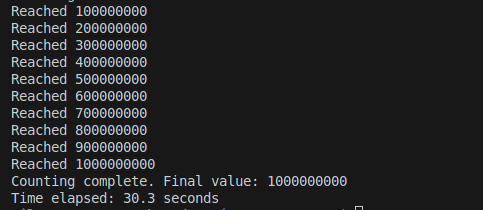
\includegraphics[width=0.8\textwidth]{../sync_records/results_java/result_1.png}
    \caption{First run of synchronous Java code execution.}
    \label{fig:Java-runtime-1}
\end{figure}

\begin{figure}[htbp]
    \centering
    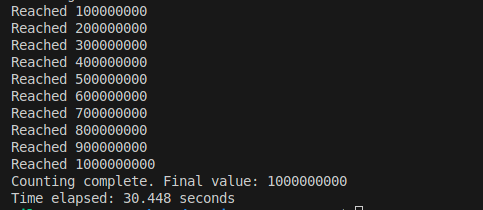
\includegraphics[width=0.8\textwidth]{../sync_records/results_java/result_2.png}
    \caption{Second run of synchronous Java code execution.}
    \label{fig:Java-runtime-2}
\end{figure}

\begin{figure}[htbp]
    \centering
    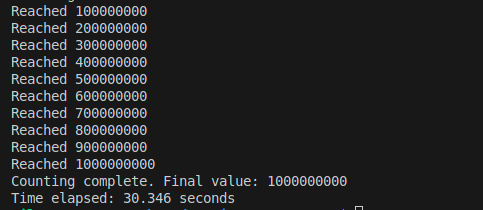
\includegraphics[width=0.8\textwidth]{../sync_records/results_java/result_3.png}
    \caption{Third run of synchronous Java code execution.}
    \label{fig:Java-runtime-3}
\end{figure}

\begin{figure}[htbp]
    \centering
    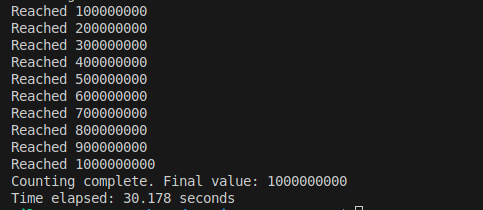
\includegraphics[width=0.8\textwidth]{../sync_records/results_java/result_4.png}
    \caption{Fourth run of synchronous Java code execution.}
    \label{fig:Java-runtime-4}
\end{figure}

\begin{figure}[htbp]
    \centering
    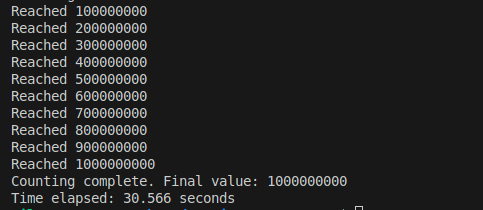
\includegraphics[width=0.8\textwidth]{../sync_records/results_java/result_5.png}
    \caption{Fifth run of synchronous Java code execution.}
    \label{fig:Java-runtime-5}
\end{figure}

\clearpage
\subsection{Python Execution Times} 

\begin{figure}[htbp]
    \centering
    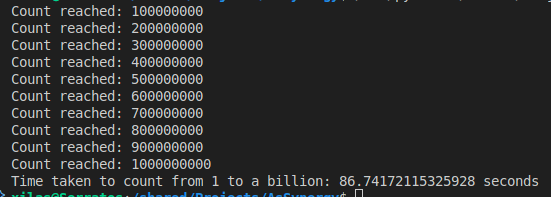
\includegraphics[width=0.8\textwidth]{../sync_records/results_python/result_1.png}
    \caption{First run of synchronous Python code execution.}
    \label{fig:Python-runtime-1}
\end{figure}

\begin{figure}[htbp]
    \centering
    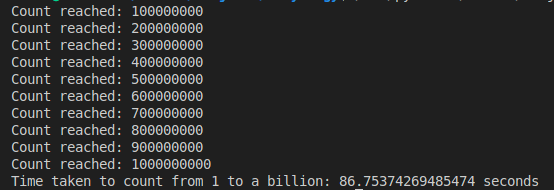
\includegraphics[width=0.8\textwidth]{../sync_records/results_python/result_2.png}
    \caption{Second run of synchronous Python code execution.}
    \label{fig:Python-runtime-2}
\end{figure}

\begin{figure}[htbp]
    \centering
    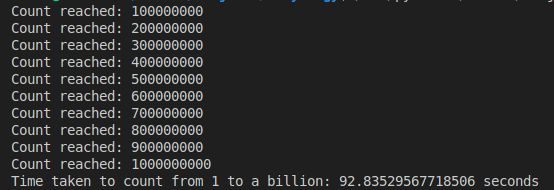
\includegraphics[width=0.8\textwidth]{../sync_records/results_python/result_3.png}
    \caption{Third run of synchronous Python code execution.}
    \label{fig:Python-runtime-3}
\end{figure}

\begin{figure}[htbp]
    \centering
    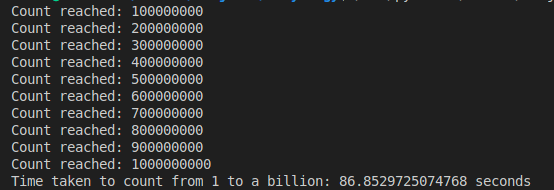
\includegraphics[width=0.8\textwidth]{../sync_records/results_python/result_4.png}
    \caption{Fourth run of synchronous Python code execution.}
    \label{fig:Python-runtime-4}
\end{figure}

\begin{figure}[htbp]
    \centering
    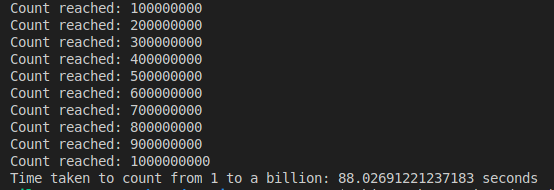
\includegraphics[width=0.8\textwidth]{../sync_records/results_python/result_5.png}
    \caption{Fifth run of synchronous Python code execution.}
    \label{fig:Python-runtime-5}
\end{figure}

\end{document}